\documentclass{sigcomm-alternate}
\usepackage[utf8]{inputenc}
\usepackage{algorithm}
\usepackage{caption}
\usepackage{subcaption}
\usepackage[noend]{algpseudocode}

\title{Minimizing Wireless Traffic Interference for User-Rich LANs With Dynamically Reconfigured Hierarchical Network Topologies}
\author{Erik Gabrielsen, Ian Johnson, Danh Nguyen, Gavin Pham, Alex Saladna, Travis Siems\\ \{egabrielsen, ianj, danhn, gpham, asaladna, tsiems\}@smu.edu}
\date{March 2016}

% Your interim draft is an early draft of your final paper, and it should be written with the end in mind. Your interim draft should be at least 3 pages in length, have the basic structure of your final paper including most, if not all, of your references, and it should have all the non-experiment dependent sections written to a draft level of understandability.
% A typical research paper has six sections plus an abstract. Generically, the six sections are: Introduction, Related Work, Research Approach, Experiment and Results, Analysis, and Conclusions (note that Conclusions is plural). The abstract plus the first three and one-half sections should be written in your interim draft. Note that poorly written is fine at this point. This is simply an early draft. There may also be holes in this draft. For example, the Introduction section should give a 30,000 foot view of your approach to solving the problem plus the primary results and conclusions. You may not have all of this information after only one month of working on your research. This is OK.

% AN EXAMPLE OF A SIGCOMM PAPER: http://www.sigcomm.org/sites/default/files/ccr/papers/2014/July/0000000-0000004.pdf

\usepackage{natbib}
\usepackage{graphicx}

\begin{document}

\maketitle

\begin{abstract}
Erik Got dis 
\end{abstract}

\section{Introduction}
Local Area Networks (LANs) which operate over a wireless medium using variants of the 802.11 protocol provide remarkable utility to users by allowing them to connect and disconnect from a network at any time without forming their own ad-hoc network to communicate with nearby users. To achieve such functionality, LANs typically operate by connecting each new user to a statically assigned physical access point (AP) which routes the user's traffic to the rest of the network. LANs often consist of tens or hundreds of users who share the wireless link among themselves using a variety of Media Access Control (MAC) algorithms and bandwidth distribution strategies such as Frequency Division Multiplexing (FDM) and Code Division Multiple Access (CDMA). While these approaches efficiently distribute network resources among nodes in a low or medium traffic density network, they deteriorate rapidly in high host/traffic density (user-rich) LANS. In all existing MAC algorithms, successful frame throughput declines significantly as host and traffic density increases on the network. Likewise, static multiplexing strategies such as FDMA and CDMA have performance issues in high-density wireless networks. 

There is, however, a third viable approach to throughput optimization for user-rich LANs. Breaking down a large LAN into sub-LANs which operate within their own geographic region can significantly improve the per-host efficiency of the overall LAN. This is often done in practice using multiple physical APs within the geographic span of a LAN. However, this approach statically allocates network resources, which causes it to suffer the same fate as FDMA when uneven network activity distributions occur. A dynamic approach with multiple physical APs is not realistic, however, as it would require that APs physically move around the network in response to varying network activity. Therefore, our research explores an algorithmic approach to dynamic subnetwork generation in which the physical root AP dynamically assigns network users to act as subAPs which route traffic from nearby users to the AP. 

In organizing a set of subnetworks, a number of considerations must be taken into account. If an algorithm is to be considered superior to the typical existing star topology, in which all hosts connect directly to a physical AP, it must outperform the star topology in most, if not all network viability metrics for a wide variety of possible network distributions. A typical LAN may be geographically organized in a normal or pseudo-random distribution, where hosts have no tendency to gravitate toward one another, or they may exist in a clustered distribution wherein hosts tend to group together. To entertain the idea of a clustered distribution, consider two scenarios. The first is a static clustering distribution, where users gravitate around a physical landmark within the geographic span of a LAN. An example of such a scenario would be an area of seats at a gate at an airport. A LAN operating in an airport is likely a user-rich LAN, and users tend to cluster together around seating areas which do not change over time. A second scenario is a dynamically clustered distribution, where the geographic location of a cluster is subject to change over time. An example would be a large conference room, wherein people move around in groups while each of their phones continuously talk to an AP. The two scenarios will be treated as one agglomerate 'clustered' distribution for the purposes of our research.

After exploring existing approaches to throughput optimization via multiplexing, MAC algorithms, and network topology optimization, we will define our model for assessing topology viability and explore the behaviour of a number of algorithms used to organize a hierarchical network topology.

\textbf{Related Work}
Cite and explain at least one paper about multiplexing strategies (e.g. FDM)

Cite and explain at least one paper about a MAC algorithm (e.g. the Aloha paper)

Cite and explain at least one paper about a LAN topology algorithm. We'll implement this/these algorithm and compare it to our results. (e.g. Prim's algorithm)

Cite AT LEAST 5 works.



\section{Topology Viability Model}
In order to ascertain the viability of a LAN topology, our model considers a set of possible geographic host distributions ranging from randomized distributions to heavily clustered distributions, as well as a variety of average host densities per geographic area which have been discretized into three categories: low, medium, and high-density. While our focus lies in the performance of LAN topology algorithms in high-density (user-rich) LANs, a viable algorithm must also provide competitive functionality compared to other algorithms in low and medium-density host distributions.

Our model operates under a set of assumptions which streamline the process of assessing the viability of topology algorithms.
\begin{itemize}
    \item \textbf{Constant transmission rates:} All hosts send data across the network at a constant rate. In practice, this rate would be the average data transmission rate of a host.
    \item \textbf{Single access point:} All hosts connect, either directly or indirectly, to a single root AP. Because each algorithm tested (excluding the null algorithm, the star topology) generates a hierarchical topology, it is assumed that each algorithm could be reasonably extended to a multi-AP system.
    \item \textbf{Mutable NIC broadcast range:} All NICs can change the power/range with which they transmit a broadcast signal. The lack of this assumption precludes any significant interference minimization.
    \item \textbf{Hosts within range of AP:} All hosts on the LAN are within range of the AP such that each host can broadcast a signal with sufficient strength to reach the AP and the AP, in turn, can broadcast a signal with sufficient strength to reach each host.
\end{itemize}

Provided this set of assumptions, our model measures the viability of an algorithm for any given environment based on a number of topology performance metrics.
\begin{itemize}
    \item \textbf{Interfering node count:} The number of nodes whose broadcasts interfere with the communications of any given node. 
    \item \textbf{Number of re-broadcasts:} The number of nodes through which the communications of any given node are routed before reaching the AP.
    \item \textbf{Signal distance to AP:} The total distance over which signals from a host travel before eventually reaching the AP.
    \item \textbf{Total network traffic:} The total amount of communication occurring over the network at any given time. Calculated as the sum of the transmission rate of each node multiplied by the number of re-broadcasts that must occur to connect a host to the AP.
\end{itemize}

Each of these metrics will be calculated for each proposed algorithm in many possible host layout scenarios.

As a basis for comparison of topology algorithms, a star topology algorithm will be used as a null algorithm. In a star topology, each host on the network connects directly to the AP. For each topology algorithm tested, the algorithm will be used to generate a topology for 50 networks from each possible combination of semi-clustered, very-clustered, and unclustered (random) host distributions with low, medium, and high host densities.

Figure 1 shows the format in which topology viability data will be presented. The 'Layout' column refers to the geographic distribution of hosts in the form $Layout:Density$, where $layout$ is $R$ for random, $SC$ for semi-clustered and $C$ for clustered, and $density$ describes the geographic host density as $L$ for low, $M$ for medium, and $H$ for high-density. The interference, hops, distance, and traffic columns refer to the four performance metrics described above (interfering node count, number of rebroadcasts, signal distance to AP, and total network traffic, respectively).


\begin{figure}[H]
  \centering
  
    \begin{tabular}{|l || c | c | c | c|}
    \hline
    Layout & Interference & Hops & Distance & Traffic \\
    \hline
    R:L & $8.93 \pm 4.39$ & $0 \pm 0$ & $272 \pm 117$ & $168$ \\
    R:M & $29.6 \pm 11.3$ & $0 \pm 0$ & $307 \pm 115$ & $508$ \\
    R:H & $72.4 \pm 27.2$ & $0 \pm 0$ & $307 \pm 118$ & $1208$ \\
    \hline
    SC:L & $16.3 \pm 5.32$ & $0 \pm 0$ & $240 \pm 126$ & $142$ \\
    SC:M & $32.4 \pm 11.7$ & $0 \pm 0$ & $315 \pm 102$ & $450$ \\
    SC:H & $74.9 \pm 27.8$ & $0 \pm 0$ & $287 \pm 103$ & $1280$ \\
    \hline
    C:L & $17.7 \pm 5.69$ & $0 \pm 0$ & $307 \pm 140$ & $127$ \\
    C:M & $40.7 \pm 15.9$ & $0 \pm 0$ & $289 \pm 101$ & $528$ \\
    C:H & $71.2 \pm 30.9$ & $0 \pm 0$ & $346 \pm 144$ & $1252$ \\
    \hline
    \end{tabular}
  
  \caption{Viability metrics for the null algorithm}
\end{figure}



\section{Proximity Greedy Algorithm}
Our first approach to generating an ideal network topology is to prioritize nodes geographically proximate to the AP to become sub-APs. To do so, a greedy algorithm was implemented which assigns the most proximate unassigned host to become a sub-AP, and assigns the n nodes closest to the new sub-AP to be its children, where n is a load factor calculated as the total number of hosts on the network divided by the desired number of sub-APs. This approach attempts an even distribution of re-transmission loads among the hosts assigned to be sub-APs.

\subsection{Proximity Greedy Algorithm}
The most basic approach to topology optimization is with an un-optimized, single-iteration of the proximity greedy algorithm. This basic proximity algorithm, when tested against a set of geographic host layouts generated according to the specifications layed out in the previous section, generated network topologies whose relevant metrics are shown in figure 2.

\begin{figure}[H]
  \centering
  
    \begin{tabular}{|l || c | c | c | c|}
    \hline
    Layout & Interference & Hops & Distance & Traffic \\
    \hline
    R:L & $4.73 \pm 3.27$ & $0.76 \pm 0.42$ & $381 \pm 112$ & $238$ \\
    R:M & $9.34 \pm 9.34$ & $0.81 \pm 0.39$ & $350 \pm 149$ & $893$ \\
    R:H & $15.9 \pm 22.2$ & $0.86 \pm 0.35$ & $332 \pm 128$ & $2300$ \\
    \hline
    SC:L & $6.11 \pm 4.77$ & $0.77 \pm 0.42$ & $316 \pm 166$ & $281$ \\
    SC:M & $10.9 \pm 10.9$ & $0.82 \pm 0.38$ & $361 \pm 150$ & $879$ \\
    SC:H & $19.1 \pm 27.8$ & $0.87 \pm 0.34$ & $334 \pm 122$ & $2548$ \\
    \hline
    C:L & $6.20 \pm 4.55$ & $0.80 \pm 0.40$ & $269 \pm 138$ & $294$ \\
    C:M & $10.7 \pm 10.8$ & $0.86 \pm 0.35$ & $244 \pm 100$ & $869$ \\
    C:H & $20.7 \pm 28.4$ & $0.86 \pm 0.35$ & $326 \pm 114$ & $2248$ \\
    \hline
    \end{tabular}
  
  \caption{Viability metrics for the basic proximity-greedy algorithm}
\end{figure}


\subsection{Post-Configuration Optimization}
Post-network configuration, the greedy algorithm can be optimized by having each non-subAP host switch to a new subAP if it is closer to a subAP other than its own. This slightly deteriorates the even distribution of traffic routed through each subAP which exists in the basic proximity greedy algorithm. Results for the optimized version of the proximity algorithm are shown in figure 3, and pseudocode for the optimized algorithm is shown below.

\begin{algorithm}[H]
\caption{Optimized Proximity Greedy Algorithm}
\begin{algorithmic}[H]
\Require{$hosts$ is a list of all hosts on the network, $subAPs$ is an empty list of subAPs, and $rootAP$ is the physical AP of the network}
\Procedure{buildNetwork}{$hosts, subAPs, rootAP$}
\State sort hosts by distance to rootAP
\For{$i \gets 1 \textrm{ to } k$}
\State $subAPs[i]\gets host[i]$
\EndFor
\For{$i \gets k \textrm{ to } numHosts$}
\State sort $subAPs$ by distance to $host[i]$
\State $host[i].myAP \gets subAPs[0]$
\EndFor
\EndProcedure
\end{algorithmic}
\end{algorithm}

\begin{figure}[H]
  \centering
  
    \begin{tabular}{|l || c | c | c | c|}
    \hline
    Layout & Interference & Hops & Distance & Traffic \\
    \hline
    R:L & $4.1 \pm 3.10$ & $0.67 \pm 0.47$ & $330 \pm 117$ & $266$ \\
    R:M & $7.61 \pm 9.29$ & $0.82 \pm 0.38$ & $335 \pm 134$ & $997$ \\
    R:H & $13.2 \pm 24.4$ & $0.86 \pm 0.35$ & $337 \pm 117$ & $2309$ \\
    \hline
    SC:L & $6.03 \pm 4.96$ & $0.80 \pm 0.40$ & $312 \pm 91$ & $280$ \\
    SC:M & $7.73 \pm 10.7$ & $0.83 \pm 0.38$ & $327 \pm 156$ & $937$ \\
    SC:H & $15.0 \pm 29.4$ & $0.86 \pm 0.34$ & $339 \pm 123$ & $2193$ \\
    \hline
    C:L & $7.23 \pm 7.65$ & $0.80 \pm 0.40$ & $307 \pm 121$ & $282$ \\
    C:M & $9.76 \pm 14.7$ & $0.84 \pm 0.37$ & $309 \pm 131$ & $999$ \\
    C:H & $13.5 \pm 25.4$ & $0.86 \pm 0.35$ & $243 \pm 116$ & $2302$ \\
    \hline
    \end{tabular}
  
  \caption{Viability metrics for the optimized proximity-greedy algorithm}
\end{figure}


Figure 4 shows a comparison of the two algorithms for a randomly distributed data set. The grayed-out area represents geographic regions where interference is occurring. Darker shades of gray indicate greater interference.

\begin{figure}[ht]
\centering
\begin{subfigure}{0.45\linewidth}
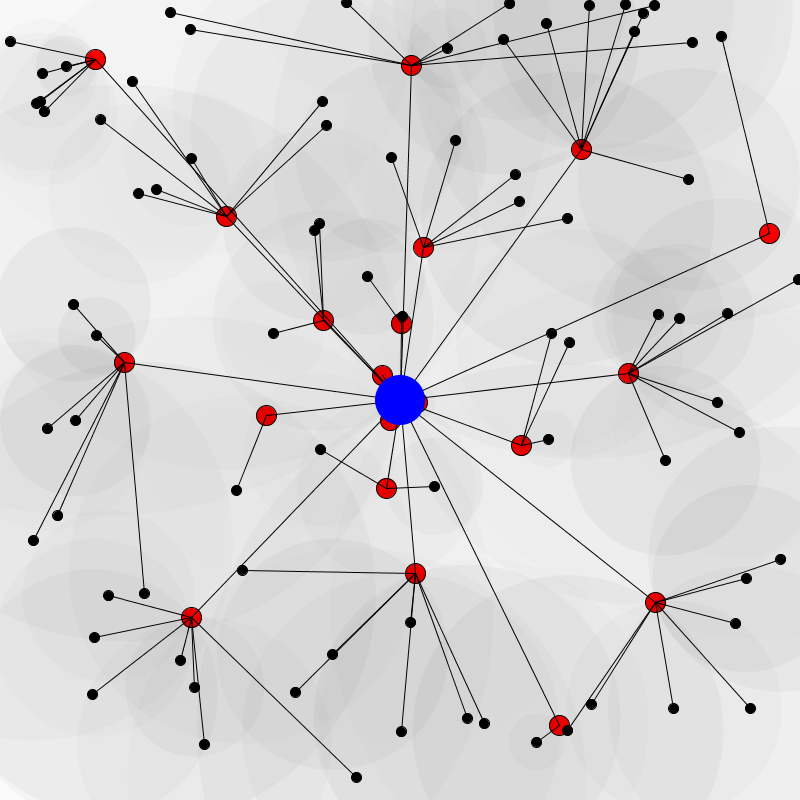
\includegraphics[scale=0.15]{UnOpt.png}
\caption{Un-Optimized}
\end{subfigure}
\quad
\begin{subfigure}{0.45\linewidth}
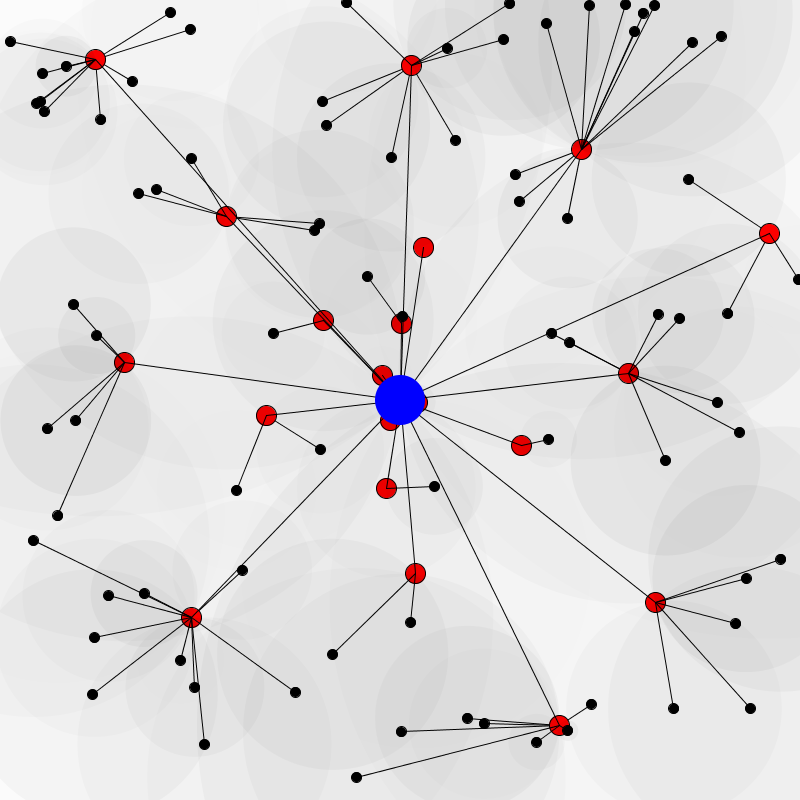
\includegraphics[scale=0.15]{opt.png}
\caption{Optimized}
\end{subfigure}
\caption{Optimized vs Un-optimized}
\end{figure}

\section{Recursive Proximity Greedy Algorithm}
As an expansion of the basic proximity greedy algorithm, two recursive versions exist which, after assigning sub-APs, allow each sub-AP to use the same proximity greedy algorithm used by the AP to assign their own sub-subAPs. Both a semi-recursive version, which restricts the network to generating a limited number of layers to the AP hierarchy, and a fully recursive version, which generates a tree of sub-APs until it reaches edge nodes on the LAN, are implemented.

\subsection{Semi-Recursive Proximity Greedy Algorithm}
In a semi-recursive approach, the proximity greedy algorithm recurses up to $k$ times to define subnetworks, sub-subnetworks, and so on. $k$ is calculated as a function of the total number of nodes on the network, such that the algorithm will recurse with depth relative to the density of the network. A viable, but less robust solution would be to simply recurse n times where n is some constant hard-coded in the algorithm. This approach, however, fails to properly scale to total number of hosts on the network. Viability metrics for the network topologies generated by this algorithm in our test environment are shown in figure 4.1.

FIGURE 4.1 -- TABLE OF STATS FOR SEMI RECURSIVE (NOT YET IMPLEMENTED ALGORITHM)

\subsection{Fully-Recursive Proximity Greedy Algorithm}
In a fully-recursive greedy approach, the proximity algorithm recurses indefinitely until it reaches edge nodes on each branch of recursion. This approach attempts to minimize total interference, not taking into account additional overhead introduced by having numerous rebroadcasts. The relevant metrics for a recursive topology algorithm are shown in figure 4.2, and pseudocode for the fully recursive algorithm is included below.

FIGURE 4.2 -- TABLE OF STATS FOR FULLY RECURSIVE (ERIK ALGORITHM)

\begin{algorithm}[H]
\caption{Recursive Proximity Greedy Algorithm}
\begin{algorithmic}[H]
\Require{$hosts$ is a list of all hosts on the network, $subAPs$ is an empty list of subAPs, and $rootAP$ is the physical AP of the network}
\Procedure{buildNetwork}{$hosts, subAPs, rootAP$}
\If{$length(hosts) <= 1$}
\State return
\EndIf
\State sort hosts by distance to rootAP
\For{$i \gets 1 \textrm{ to } k$}
\State $subAPs[i]\gets hosts[i]$
\EndFor
\For{$i \gets k \textrm{ to } numHosts$}
\State sort $subAPs$ by distance to $hosts[i]$
\State $hosts[i].myAP \gets subAPs[0]$
\State $subAPs[0].myChildren.append(hosts[i])$
\EndFor
\For{$subAP$ in $subAPs$}
\State buildNetwork($subAP.myChildren$, $[]$, $subAP$)
\EndFor
\EndProcedure
\end{algorithmic}
\end{algorithm}

Figure N shows a topology generated by a fully-recursive distance greedy algorithm. The resulting network has very low interference, but a high number of re-broadcasts must occur to transfer information from edge nodes to the AP.

\begin{figure}[H]
\centering
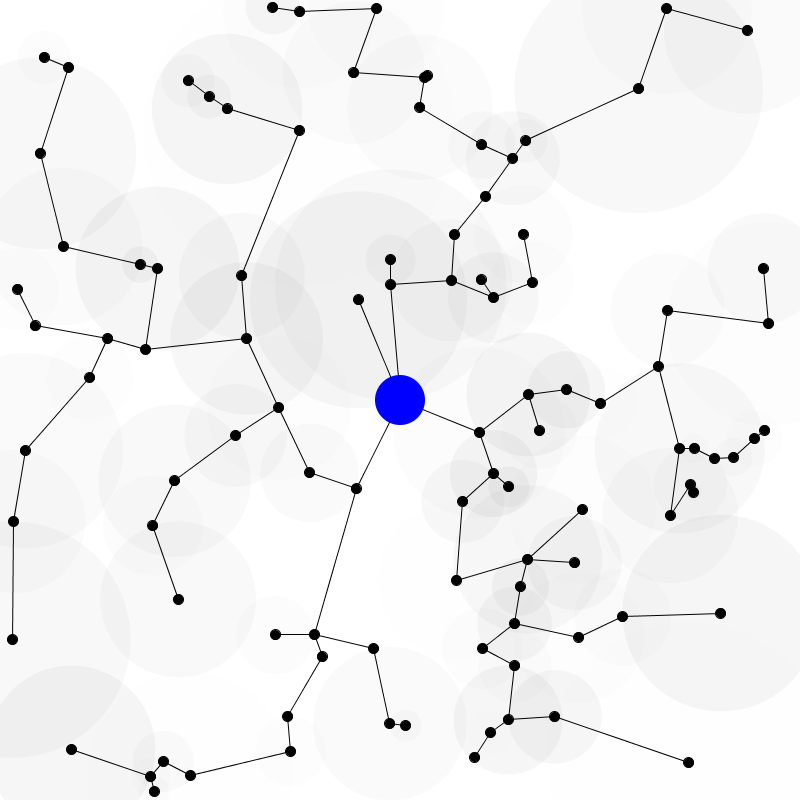
\includegraphics[scale=0.15]{erikFullyRecursive.png}
\caption{Optimized vs Un-optimized}
\end{figure}

\section{Centralization Greedy Algorithm}
In order to optimize for areas of high host density which are isolate from the location of the AP, a greedy algorithm is implemented which selects sub-APs based on hosts' centralization relative to all other hosts on the network, where centralization is defined as the average distance to each other host on the network from any given node. This is implemented as a single-tier hierarchy as well as a recursive multi-tier hierarchy.

\subsection{Single-Tier Centralization}
In a single-tier centralization approach, a single iteration of the centralization greedy algorithm assigns $k$ sub-APs based on highest overall proximity where $k$ is a function of the total number of hosts on the network. Figure 5.1 shows topology viability metrics for an implementation of this single-tier centralization greedy algorithm.

FIGURE 5.1 -- TABLE OF STATS FOR IAN ALGORITHM

\subsection{Multi-Tier Centralization}
In a multi-tier centralization approach, the centralization greedy algorithm recurses up to $\log_2 k$, where $k$ is a function of the total number of hosts on the network, and on layer n of recursion, the algorithm assigns $\frac{k}{2^n}$ subAPs, where $n = 0$ at the first layer of recursion. Results from the multi-tier centralization algorithm can be found in figure 5.2, and pseudocode for the algorithm is shown below.

FIGURE 5.2 -- TABLE OF STATS FOR RECURSIVE IAN ALGORITHM

\begin{algorithm}[H]
\caption{Recursive Centralization Greedy Algorithm}
\begin{algorithmic}[H]
\Require{$hosts$ is a list of all hosts on the network, $subAPs$ is an empty list of subAPs}
\Procedure{buildNetwork}{$hosts, subAPs$}
\State sort hosts by centralization
\For{$i \gets 1 \textrm{ to } k$}
\State $subAPs[i]\gets host[i]$
\EndFor
\For{$i \gets k \textrm{ to } numHosts$}
\State sort $subAPs$ by distance to $host[i]$
\State $host[i].myAP \gets subAPs[0]$
\State $subAPs[0].myChildren.append(hosts[i])$
\EndFor
\For{$subAP$ in $subAPs$}
\State buildNetwork($subAP.myChildren$, $[]$)
\EndFor
\EndProcedure
\end{algorithmic}
\end{algorithm}


Figure N shows a comparison of the two algorithms for a randomly distributed data set. While the single-tier centralization reduces interference mostly around the physical AP, the recursive version optimizes overall interference.

\begin{figure}[ht]
\centering
\begin{subfigure}{0.45\linewidth}
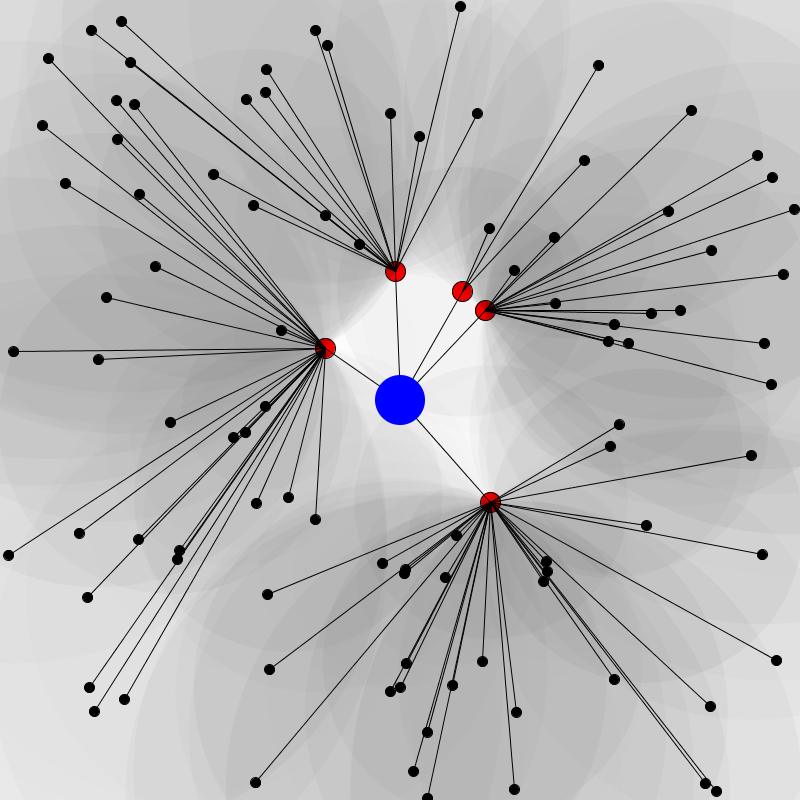
\includegraphics[scale=0.15]{ianNotRecursive.png}
\caption{Un-Optimized}
\end{subfigure}
\quad
\begin{subfigure}{0.45\linewidth}
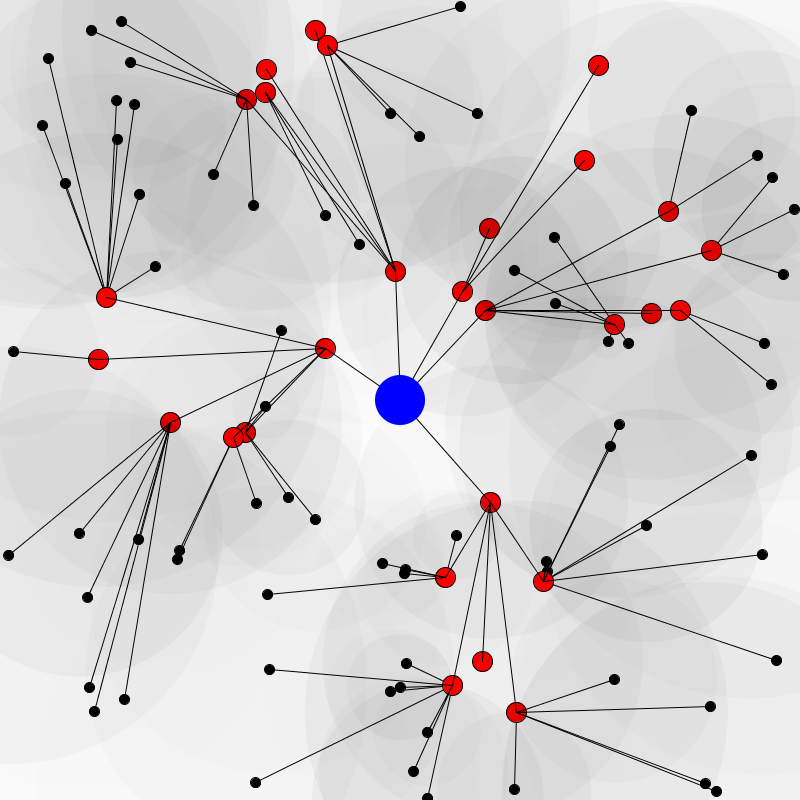
\includegraphics[scale=0.15]{ianRecursive.png}
\caption{Optimized}
\end{subfigure}
\caption{Single vs Multi-tier centralization}
\end{figure}

\bibliographystyle{plain}
\bibliography{references}

%For previous work:
%http://www.ijser.org/researchpaper%5CA-REVIEW-PAPER-ON-ORTHOGONAL-FREQUENCY-DIVISION.pdf
%http://www.ece.umn.edu/~nihar/papers/ICC-paper-Mariam.pdf
%http://users.ece.utexas.edu/~gerstl/publications/iess13.prims.pdf
%http://www.macs.hw.ac.uk/~isi3/Phd_Proposal_files/Phd_draftproposal%5b3%5d.pdf
%Tentative on below essay
%http://www.isprs.org/proceedings/XXXVIII/7-C4/313_GSEM2009.pdf

\end{document}
